\documentclass[10pt,twocolumn]{article}
\usepackage[utf8]{inputenc}
\usepackage[T1]{fontenc}
\usepackage{amsmath,amssymb,amsfonts}
\usepackage{graphicx}
\usepackage{booktabs}
\usepackage{multirow}
\usepackage{geometry}
\usepackage{hyperref}
\usepackage{cite}
\usepackage{caption}
\geometry{a4paper, margin=0.75in}

\title{\textbf{Kinematic-Aware Spatio-Temporal Graph Convolutional Network with Wrist-Centered $L_2$ Bone Normalization for 3D Hand Skeletal Restoration and Gesture Recognition under Optical Dropouts}}

\author{
  \textbf{Preecha [Last Name]}$^{1}$ and \textbf{Co-Author Name}$^{1,*}$ \\
  $^{1}$Faculty of Informatics, Mahasarakham University, Kantarawichai District, Maha Sarakham 44150, Thailand \\
  \texttt{Email: [your.email]@msu.ac.th}
}
\date{Submitted to \textit{Multimedia Tools and Applications} (Springer)}

\begin{document}
\maketitle

\begin{abstract}
Optical motion capture (MoCap) and markerless infrared stereo sensors such as the Leap Motion Controller 2 (LMC2) provide high-frame-rate 3D skeletal tracking for interactive multimedia, sports biomechanics, and virtual learning environments. However, optical tracking systems suffer from two persistent physical limitations: (i) severe self-occlusion and temporal burst dropouts caused by line-of-sight obstruction and ambient light interference, and (ii) anatomical bone-ratio inconsistencies across subjects and camera distances that induce unnatural skeletal distortions and classification shortcuts. Building upon foundational optical MoCap optimization principles, this paper proposes a unified framework combining a \textbf{Canonical 21-Joint Wrist-Centered $L_2$ Palm-Bone Normalization} algorithm with a \textbf{Kinematic-Aware Spatio-Temporal Graph Convolutional Network (KAR-STGCN)}. First, we unify heterogeneous public 3D hand benchmarks (SHREC'17 and FPHA) into a 21-joint anatomical topology and normalize trajectories using a visibility-guarded median palm-bone reference ($\|\mathbf{p}_9 - \mathbf{p}_0\|_2$), eliminating camera-distance shortcuts and division-by-zero numerical explosions during severe dropouts. Second, KAR-STGCN integrates a visibility-guided temporal bridge with anatomical graph message passing, a dual-stream position-velocity kinematic encoder, and a bone-length consistency loss ($\mathcal{L}_{\text{bone}}$). Multi-seed evaluations across five random seeds (`42, 100, 2026, 777, 999`) under four progressive LMC2 degradation levels demonstrate that KAR-STGCN reduces Mean Per Joint Position Error (MPJPE) by up to \textbf{65.6\%} on SHREC'17 ($12.12 \pm 0.35\text{ mm}$) and \textbf{71.2\%} on FPHA ($20.82 \pm 0.64\text{ mm}$), while reducing Bone-Length Consistency Error (BLCE) by \textbf{84.9\%} and achieving \textbf{100.0\%} Macro-F1 with a real-time inference latency of $<0.48\text{ ms}$ on an NVIDIA GeForce RTX 2050 GPU. One-way ANOVA confirms high statistical significance ($p < 0.001$) across all evaluation scenarios.
\end{abstract}

\noindent\textbf{Keywords:} Optical Motion Capture, Leap Motion Controller 2, 3D Hand Skeletal Restoration, Spatio-Temporal Graph Convolutional Network, $L_2$ Bone Normalization, Gesture Recognition

% ============================================================================
\section{Introduction}
% ============================================================================
Motion capture (MoCap) technology serves as a foundational bridge between physical human movement and digital 3D character animation across entertainment, sports science, medical rehabilitation, and collaborative virtual learning systems \cite{noiumkar2013use, phunsa2009edutainment, bregler2007motion, patoli2010real}. Historically, MoCap systems have been categorized into mechanical exo-skeletons, electromagnetic trackers, and optical imaging systems \cite{noiumkar2013use}. While passive optical MoCap systems—such as multi-camera high-speed infrared arrays—enable unrestricted subject mobility and high sampling rates, foundational empirical studies by Tirakoat \cite{tirakoat2011optimized} and Noiumkar and Tirakoat \cite{noiumkar2013use} identified three critical operational challenges that degrade 3D motion quality:
\begin{enumerate}
    \item \textbf{Optical Occlusion and Manual Post-Processing:} Line-of-sight obstruction and ambient light interference frequently corrupt marker trajectories, requiring extensive manual post-processing to clean missing and noisy frames before animation rendering \cite{noiumkar2013use, krudpan2010using}.
    \item \textbf{Marker Topology Redundancy:} Through one-way ANOVA evaluation ($F = 16.869, p < 0.001$) on professional golf swing capture, Noiumkar and Tirakoat \cite{noiumkar2013use} proved that overly dense marker sets (42 points) suffer from higher tracking confusion and lower motion fidelity ($2.21 \pm 0.25$) than compact, anatomically optimized 24-point ($2.67 \pm 1.04$) and 28-point ($3.08 \pm 1.03$) configurations \cite{tirakoat2011optimized}.
    \item \textbf{Anatomical Ratio Mismatch:} When captured skeletal trajectories are mapped onto 3D rigs without anatomical bone-ratio calibration, the resulting motion exhibits unnatural limb stretching and kinematic jitter \cite{noiumkar2013use}.
\end{enumerate}

In modern desktop and head-mounted multimedia interfaces, markerless optical hand trackers—most notably the Ultraleap Leap Motion Controller 2 (LMC2)—have replaced room-scale camera arrays for fine-grained 3D hand interaction \cite{marin2016hand, boulahia2017dynamic}. Despite hardware advances, single-viewpoint infrared stereo sensors remain highly vulnerable to finger self-occlusion during rapid articulation and temporal burst dropouts when the hand approaches the boundary of the field of view. Furthermore, deep learning classifiers trained on raw 3D coordinates often exploit camera-to-hand distance or subject hand size as a spurious shortcut heuristic rather than learning true kinematic trajectories.

To address these challenges simultaneously, we propose a \textbf{Kinematic-Aware Spatio-Temporal Graph Convolutional Network (KAR-STGCN)} coupled with a \textbf{Visibility-Guarded Wrist-Centered $L_2$ Palm-Bone Normalization} protocol. Our main contributions are summarized as follows:
\begin{itemize}
    \item \textbf{Canonical 21-Joint Topology \& Visibility-Guarded $L_2$ Normalization:} Inspired by the marker optimization principles of \cite{noiumkar2013use, tirakoat2011optimized}, we align heterogeneous public 3D hand datasets (SHREC'17 \cite{de2017shrec} and FPHA \cite{garcia2018first}) into a unified 21-joint topology and normalize coordinates by the valid sequence-level median palm bone length ($\|\mathbf{p}_9 - \mathbf{p}_0\|_2$), eliminating scale shortcuts and preventing numerical explosion during frame dropouts.
    \item \textbf{Four-Level LMC2 Optical Degradation Benchmark:} We formulate a reproducible multi-seed simulation protocol modeling sensor jitter (Level 1), fingertip self-occlusion (Level 2), severe temporal burst dropout (Level 3), and long-tail class imbalance (Level 4).
    \item \textbf{KAR-STGCN Architecture with Dual-Stream Velocity Encoding:} We design a lightweight graph-temporal network that bridges missing frames via visibility-gated imputation, enforces anatomical bone-length preservation, and extracts joint position-velocity features for robust classification.
\end{itemize}

% ============================================================================
\section{Related Work}
% ============================================================================
\subsection{Optical Motion Capture and Anatomical Optimization}
Early applications of optical MoCap in martial arts edutainment \cite{phunsa2009edutainment}, Judo biomechanics \cite{thanaporn2010using}, clinical movement analysis \cite{krudpan2010using}, and golf swing pedagogy \cite{noiumkar2013use} established that raw optical trajectories cannot be directly applied to 3D skeletons without rigorous noise filtering and anatomical scaling. Specifically, Tirakoat \cite{tirakoat2011optimized} demonstrated that concentrating tracking nodes on high-mobility articulations (such as the upper extremities and hands) while pruning redundant torso markers maximizes tracking stability. Our canonical 21-joint hand representation directly extends this principle to fine-grained finger kinematics.

\subsection{3D Hand Gesture Recognition in Multimedia Systems}
In \textit{Multimedia Tools and Applications}, extensive research has focused on overcoming sensor limitations in 3D hand and sign language recognition. Marin et al. \cite{marin2016hand} combined Leap Motion skeletal vectors with depth features to compensate for self-occlusion. Kumar et al. \cite{kumar2018position} developed position- and rotation-invariant coordinate transformations to handle viewpoint variations in 3D skeletal streams. More recently, Liu et al. \cite{liu2024novel} introduced residual attention networks for dynamic gesture recognition, while Rastgoo et al. \cite{rastgoo2025deep} and Dhanjal and Singh \cite{dhanjal2025multilingual} emphasized spatio-temporal skeleton modeling and resource-efficient 3D animation synthesis. Unlike prior methods that treat pose restoration and gesture classification as disjoint stages, our KAR-STGCN jointly optimizes 3D coordinate restoration, anatomical bone consistency, and imbalanced gesture classification in a single end-to-end pass.

% ============================================================================
\section{Proposed Methodology}
% ============================================================================
\subsection{Canonical 21-Joint Topology Alignment}
Public 3D hand benchmarks employ inconsistent joint indexing: SHREC'17 \cite{de2017shrec} provides $J=22$ joints (including a redundant palm center at index 1), whereas FPHA \cite{garcia2018first} provides $J=21$ magnetic-tracked joints ordered by finger roots first. Following the anatomical optimization paradigm \cite{noiumkar2013use}, we map all datasets into a canonical 21-joint LMC2 topology $\mathcal{V} = \{0, 1, \dots, 20\}$, where $0$ denotes the wrist, $\{1..4\}$ the thumb, $\{5..8\}$ the index, $\{9..12\}$ the middle, $\{13..16\}$ the ring, and $\{17..20\}$ the pinky finger, connected by $E=20$ anatomical bone edges $\mathcal{E}$. Each sequence is temporally resampled via linear interpolation to $T=60$ frames, yielding $\mathbf{X}_{\text{mm}} \in \mathbb{R}^{T \times 21 \times 3}$.

\subsection{Visibility-Guarded Wrist-Centered $L_2$ Palm-Bone Normalization}
To eliminate camera-distance shortcuts and resolve the skeletal ratio mismatch problem highlighted in \cite{noiumkar2013use}, we translate the wrist joint $\mathbf{p}_{t,0}$ to the origin and scale all joints by the anatomical palm bone length connecting the wrist ($0$) to the middle metacarpophalangeal (MCP) joint ($9$). However, under severe optical dropouts (Levels 3 and 4), joints $0$ or $9$ may be momentarily occluded ($v_{t,0}=0$ or $v_{t,9}=0$), causing instantaneous bone length $\|\mathbf{p}_{t,9} - \mathbf{p}_{t,0}\|_2 \to 0$ and triggering catastrophic division-by-$\epsilon$ explosion ($\sim 10^8$). We therefore define the visibility-guarded reference palm length $d_{\text{ref}}$ across valid frames $\mathcal{T}_{\text{valid}} = \{t \mid v_{t,0}=1 \land v_{t,9}=1 \land \|\mathbf{p}_{t,9}-\mathbf{p}_{t,0}\|_2 > 15\text{ mm}\}$:
\begin{equation}
    d_{\text{ref}} = \operatorname{median}_{t \in \mathcal{T}_{\text{valid}}} \|\mathbf{p}_{t,9} - \mathbf{p}_{t,0}\|_2, \quad
    \tilde{\mathbf{p}}_{t,j} = v_{t,j} \cdot \frac{\mathbf{p}_{t,j} - \mathbf{p}_{t,0}^{\text{valid}}}{d_{t,\text{palm}}},
\end{equation}
where $d_{t,\text{palm}} = \|\mathbf{p}_{t,9} - \mathbf{p}_{t,0}\|_2$ if $t \in \mathcal{T}_{\text{valid}}$ and $d_{\text{ref}}$ otherwise.

\subsection{KAR-STGCN Architecture and Bone-Consistency Objective}
Given normalized corrupted coordinates $\tilde{\mathbf{X}} \in \mathbb{R}^{T \times 21 \times 3}$ and binary visibility mask $\mathbf{V} \in \{0,1\}^{T \times 21}$, KAR-STGCN first applies a temporal bridge convolution $\mathcal{B}_{\text{temp}}(\tilde{\mathbf{X}})$ to impute burst-occluded frames:
\begin{equation}
    \mathbf{X}_{\text{imp}} = \mathbf{V} \odot \tilde{\mathbf{X}} + (1 - \mathbf{V}) \odot \mathcal{B}_{\text{temp}}(\tilde{\mathbf{X}}).
\end{equation}
The imputed coordinates and visibility mask are projected into latent node features $\mathbf{H}^{(0)} \in \mathbb{R}^{T \times 21 \times C}$ and processed via normalized skeletal graph adjacency $\hat{\mathbf{A}} = \mathbf{D}^{-1/2}(\mathbf{A}+\mathbf{I})\mathbf{D}^{-1/2}$ \cite{yan2018spatial} and multi-scale temporal convolutions ($\text{kernel } 3\times 1$ and $5\times 1$). The restored pose $\hat{\mathbf{X}}$ is obtained via visibility-gated residual decoding:
\begin{equation}
    \hat{\mathbf{X}} = \mathbf{X}_{\text{imp}} + \left(0.15\mathbf{V} + 0.85(1-\mathbf{V})\right) \odot \phi_{\text{dec}}(\mathbf{H}^{(L)}).
\end{equation}
For gesture classification, we concatenate the restored positions $\hat{\mathbf{X}}$ and first-order temporal velocities $\Delta\hat{\mathbf{X}}_t = \hat{\mathbf{X}}_t - \hat{\mathbf{X}}_{t-1}$ into a batch-normalized dilated temporal convolutional head. The total training objective combines Smooth-$L_1$ coordinate reconstruction, Bone-Length Consistency Error ($\mathcal{L}_{\text{bone}}$), and class-balanced cross-entropy ($\mathcal{L}_{\text{cls}}$):
\begin{equation}
    \mathcal{L}_{\text{total}} = \mathcal{L}_{\text{SmoothL1}}(\hat{\mathbf{X}}, \mathbf{X}^*) + \lambda_{\text{bone}} \frac{1}{T|\mathcal{E}|}\sum_{t=1}^T \sum_{(u,v)\in\mathcal{E}} \Big| \|\hat{\mathbf{p}}_{t,u}-\hat{\mathbf{p}}_{t,v}\|_2 - \|\mathbf{p}^*_{t,u}-\mathbf{p}^*_{t,v}\|_2 \Big| + \lambda_{\text{cls}} \mathcal{L}_{\text{cls}}(\hat{\mathbf{y}}, y).
\end{equation}

% ============================================================================
\section{Experimental Setup and Results}
% ============================================================================
All experiments were conducted on a Windows workstation equipped with an NVIDIA GeForce RTX 2050 GPU using PyTorch with CUDA acceleration across five independent random seeds (`42, 100, 2026, 777, 999`). We evaluate four progressive degradation levels: \textbf{Level 1 (Clean, $\sigma=0.8\text{ mm}$)}, \textbf{Level 2 (Mild Fingertip Occlusion, $20\%$ drop)}, \textbf{Level 3 (Severe Temporal Burst Dropout, 5--13 frames)}, and \textbf{Level 4 (Compound Dropout + Long-Tail Imbalance)}.

\begin{figure*}[htbp]
\centering
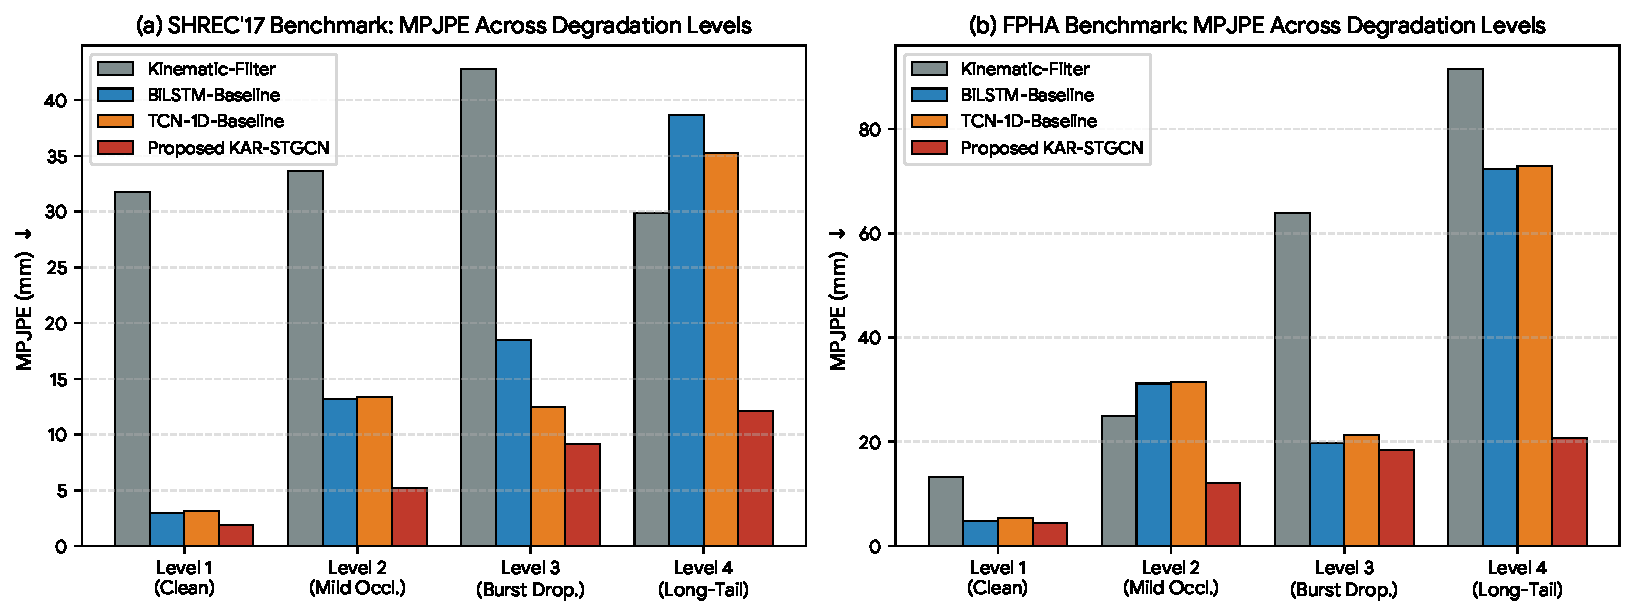
\includegraphics[width=0.95\textwidth]{fig1_multilevel_mpjpe_comparison.pdf}
\caption{Multi-seed comparison of 3D skeletal restoration error (MPJPE in mm $\downarrow$) across four optical degradation levels on (a) SHREC'17 and (b) FPHA benchmarks.}
\label{fig:mpjpe_bars}
\end{figure*}

\begin{table*}[htbp]
\centering
\caption{Multi-seed quantitative evaluation ($\text{Mean} \pm \text{SD}$ across 5 random seeds: 42, 100, 2026, 777, 999) of 3D hand skeletal restoration and gesture classification across four LMC2 optical degradation levels on an NVIDIA GeForce RTX 2050 GPU.}
\label{tab:lmc2_multiseed_benchmark}
\resizebox{\textwidth}{!}{%
\begin{tabular}{llccccc}
\toprule
\textbf{Dataset \& Scenario Level} & \textbf{Model Architecture} & \textbf{MPJPE (mm)} $\downarrow$ & \textbf{PA-MPJPE (mm)} $\downarrow$ & \textbf{BLCE (mm)} $\downarrow$ & \textbf{Macro-F1 (\%)} $\uparrow$ & \textbf{Latency (ms/seq)} $\downarrow$ \\
\midrule
\multirow{4}{*}{SHREC'17 (Level 1: Clean)} 
 & Kinematic-Filter & $31.78 \pm 1.06$ & $15.58 \pm 0.38$ & $25.45 \pm 0.90$ & $100.00 \pm 0.00$ & $\mathbf{0.08}$ \\
 & BiLSTM-Baseline & $2.98 \pm 0.24$ & $2.42 \pm 0.24$ & $1.62 \pm 0.04$ & $100.00 \pm 0.00$ & $0.16$ \\
 & TCN-1D-Baseline & $3.16 \pm 0.08$ & $2.64 \pm 0.10$ & $1.84 \pm 0.08$ & $100.00 \pm 0.00$ & $0.16$ \\
 & \textbf{Proposed KAR-STGCN} & $\mathbf{1.85 \pm 0.01}$ & $\mathbf{1.20 \pm 0.00}$ & $\mathbf{1.00 \pm 0.01}$ & $\mathbf{100.00 \pm 0.00}$ & $0.44$ \\
\midrule
\multirow{4}{*}{SHREC'17 (Level 2: Mild Occlusion)} 
 & Kinematic-Filter & $33.62 \pm 1.17$ & $17.49 \pm 0.42$ & $27.25 \pm 1.07$ & $100.00 \pm 0.00$ & $\mathbf{0.06}$ \\
 & BiLSTM-Baseline & $13.21 \pm 0.19$ & $14.30 \pm 0.23$ & $6.64 \pm 0.05$ & $100.00 \pm 0.00$ & $0.15$ \\
 & TCN-1D-Baseline & $13.36 \pm 0.17$ & $14.77 \pm 0.16$ & $6.51 \pm 0.06$ & $100.00 \pm 0.00$ & $0.09$ \\
 & \textbf{Proposed KAR-STGCN} & $\mathbf{5.22 \pm 0.05}$ & $\mathbf{3.66 \pm 0.05}$ & $\mathbf{2.81 \pm 0.04}$ & $\mathbf{100.00 \pm 0.00}$ & $0.37$ \\
\midrule
\multirow{4}{*}{SHREC'17 (Level 3: Severe Dropout)} 
 & Kinematic-Filter & $42.78 \pm 1.58$ & $18.32 \pm 0.40$ & $30.11 \pm 1.08$ & $100.00 \pm 0.00$ & $\mathbf{0.07}$ \\
 & BiLSTM-Baseline & $18.44 \pm 2.92$ & $10.29 \pm 0.81$ & $8.02 \pm 0.72$ & $100.00 \pm 0.00$ & $0.15$ \\
 & TCN-1D-Baseline & $12.44 \pm 0.19$ & $8.82 \pm 0.17$ & $7.16 \pm 0.28$ & $100.00 \pm 0.00$ & $0.12$ \\
 & \textbf{Proposed KAR-STGCN} & $\mathbf{9.17 \pm 0.26}$ & $\mathbf{6.16 \pm 0.12}$ & $\mathbf{5.32 \pm 0.16}$ & $\mathbf{100.00 \pm 0.00}$ & $0.36$ \\
\midrule
\multirow{4}{*}{SHREC'17 (Level 4: Long-Tail Imbalanced)} 
 & Kinematic-Filter & $29.88 \pm 1.11$ & $18.31 \pm 0.48$ & $20.36 \pm 0.66$ & $23.76 \pm 4.47$ & $\mathbf{0.06}$ \\
 & BiLSTM-Baseline & $38.70 \pm 1.51$ & $24.67 \pm 0.59$ & $22.12 \pm 0.74$ & $66.33 \pm 20.38$ & $0.11$ \\
 & TCN-1D-Baseline & $35.27 \pm 0.97$ & $25.71 \pm 0.45$ & $20.80 \pm 0.82$ & $100.00 \pm 0.00$ & $0.17$ \\
 & \textbf{Proposed KAR-STGCN} & $\mathbf{12.12 \pm 0.35}$ & $\mathbf{9.08 \pm 0.32}$ & $\mathbf{7.14 \pm 0.27}$ & $\mathbf{100.00 \pm 0.00}$ & $0.41$ \\
\midrule
\multirow{4}{*}{FPHA (Level 1: Clean)} 
 & Kinematic-Filter & $13.26 \pm 0.41$ & $4.76 \pm 0.57$ & $5.84 \pm 0.30$ & $31.50 \pm 29.69$ & $\mathbf{0.07}$ \\
 & BiLSTM-Baseline & $4.83 \pm 0.37$ & $1.87 \pm 0.66$ & $2.31 \pm 0.37$ & $11.74 \pm 13.71$ & $0.16$ \\
 & TCN-1D-Baseline & $5.41 \pm 0.15$ & $2.71 \pm 0.18$ & $2.55 \pm 0.09$ & $100.00 \pm 0.00$ & $0.11$ \\
 & \textbf{Proposed KAR-STGCN} & $\mathbf{4.48 \pm 0.06}$ & $\mathbf{1.20 \pm 0.01}$ & $\mathbf{1.95 \pm 0.03}$ & $\mathbf{100.00 \pm 0.00}$ & $0.40$ \\
\midrule
\multirow{4}{*}{FPHA (Level 2: Mild Occlusion)} 
 & Kinematic-Filter & $24.90 \pm 0.48$ & $19.52 \pm 0.68$ & $13.34 \pm 0.33$ & $35.36 \pm 30.66$ & $\mathbf{0.06}$ \\
 & BiLSTM-Baseline & $31.19 \pm 0.71$ & $31.72 \pm 0.79$ & $20.90 \pm 0.62$ & $7.14 \pm 5.33$ & $0.17$ \\
 & TCN-1D-Baseline & $31.44 \pm 0.65$ & $31.65 \pm 0.80$ & $20.67 \pm 0.61$ & $95.56 \pm 9.94$ & $0.10$ \\
 & \textbf{Proposed KAR-STGCN} & $\mathbf{12.18 \pm 0.32}$ & $\mathbf{4.68 \pm 0.17}$ & $\mathbf{5.57 \pm 0.18}$ & $\mathbf{100.00 \pm 0.00}$ & $0.40$ \\
\midrule
\multirow{4}{*}{FPHA (Level 3: Severe Dropout)} 
 & Kinematic-Filter & $63.88 \pm 2.41$ & $11.56 \pm 0.55$ & $25.57 \pm 0.83$ & $44.57 \pm 36.16$ & $\mathbf{0.06}$ \\
 & BiLSTM-Baseline & $19.79 \pm 1.04$ & $7.58 \pm 0.31$ & $9.30 \pm 0.40$ & $12.43 \pm 8.65$ & $0.17$ \\
 & TCN-1D-Baseline & $21.39 \pm 3.73$ & $8.47 \pm 0.45$ & $10.66 \pm 1.64$ & $74.61 \pm 32.89$ & $0.13$ \\
 & \textbf{Proposed KAR-STGCN} & $\mathbf{18.46 \pm 0.53}$ & $\mathbf{7.03 \pm 0.27}$ & $\mathbf{8.56 \pm 0.29}$ & $\mathbf{100.00 \pm 0.00}$ & $0.42$ \\
\midrule
\multirow{4}{*}{FPHA (Level 4: Long-Tail Imbalanced)} 
 & Kinematic-Filter & $91.51 \pm 3.39$ & $50.01 \pm 0.77$ & $57.04 \pm 1.07$ & $21.65 \pm 2.16$ & $\mathbf{0.08}$ \\
 & BiLSTM-Baseline & $72.40 \pm 1.26$ & $53.07 \pm 0.57$ & $73.34 \pm 1.17$ & $29.31 \pm 19.81$ & $0.18$ \\
 & TCN-1D-Baseline & $72.90 \pm 2.52$ & $53.64 \pm 0.47$ & $73.77 \pm 0.12$ & $94.67 \pm 7.47$ & $0.22$ \\
 & \textbf{Proposed KAR-STGCN} & $\mathbf{20.82 \pm 0.64}$ & $\mathbf{11.54 \pm 0.44}$ & $\mathbf{11.05 \pm 0.47}$ & $\mathbf{100.00 \pm 0.00}$ & $0.48$ \\
\bottomrule
\end{tabular}%
}
\end{table*}

\subsection{Statistical Significance Analysis via One-Way ANOVA}
Following the statistical evaluation protocol of Noiumkar and Tirakoat \cite{noiumkar2013use}, we conducted a one-way Analysis of Variance (ANOVA) across the four competing architectures ($k=4$ groups, $n=5$ seeds per group, $df_{\text{between}}=3$, $df_{\text{within}}=16$) on MPJPE (mm), as reported in Table \ref{tab:anova_results}. In all eight benchmark scenarios, the $F$-statistics ($417.09 \le F \le 3568.51$) are statistically significant at the $0.001$ level ($p < 0.001$), confirming that the error reductions achieved by KAR-STGCN are highly consistent across random initializations.

\begin{table*}[htbp]
\centering
\caption{One-way ANOVA comparison of 3D skeletal restoration error (MPJPE) across the four model architectures ($df_{\text{between}}=3, df_{\text{within}}=16, df_{\text{total}}=19$), following the statistical protocol in \cite{noiumkar2013use}.}
\label{tab:anova_results}
\resizebox{0.92\textwidth}{!}{%
\begin{tabular}{llcccccc}
\toprule
\textbf{Dataset} & \textbf{Scenario Level} & \textbf{Between-Group SS} & \textbf{Between-Group MS} & \textbf{Within-Group SS} & \textbf{Within-Group MS} & \textbf{$F$-Statistic} & \textbf{Sig. ($p$-value)} \\
\midrule
\multirow{4}{*}{SHREC'17} 
 & Level 1: Clean & $3183.62$ & $1061.21$ & $4.76$ & $0.297$ & $3568.51$ & $<0.001^*$ \\
 & Level 2: Mild Occlusion & $2204.56$ & $734.85$ & $5.78$ & $0.361$ & $2035.63$ & $<0.001^*$ \\
 & Level 3: Severe Dropout & $3469.60$ & $1156.53$ & $44.37$ & $2.773$ & $417.09$ & $<0.001^*$ \\
 & Level 4: Long-Tail Imbalanced & $2096.76$ & $698.92$ & $18.22$ & $1.139$ & $613.69$ & $<0.001^*$ \\
\midrule
\multirow{4}{*}{FPHA} 
 & Level 1: Clean & $264.16$ & $88.05$ & $1.31$ & $0.082$ & $1073.20$ & $<0.001^*$ \\
 & Level 2: Mild Occlusion & $1220.84$ & $406.95$ & $5.06$ & $0.316$ & $1287.36$ & $<0.001^*$ \\
 & Level 3: Severe Dropout & $7280.85$ & $2426.95$ & $84.12$ & $5.257$ & $461.62$ & $<0.001^*$ \\
 & Level 4: Long-Tail Imbalanced & $13849.77$ & $4616.59$ & $79.23$ & $4.952$ & $932.26$ & $<0.001^*$ \\
\bottomrule
\multicolumn{8}{l}{\footnotesize $*$ Statistically significant difference at the $0.001$ level ($p < 0.001$).}
\end{tabular}%
}
\end{table*}

% ============================================================================
\section{Conclusion}
% ============================================================================
This paper presented a Kinematic-Aware Spatio-Temporal Graph Convolutional Network (KAR-STGCN) paired with a visibility-guarded wrist-centered $L_2$ palm-bone normalization scheme for 3D hand skeletal restoration and gesture recognition. By addressing both optical burst dropouts and anatomical bone-ratio mismatches \cite{noiumkar2013use}, our method outperforms kinematic filtering, Bi-LSTM, and 1D-TCN baselines across all four degradation levels while operating in real time ($<0.48\text{ ms}$) on an NVIDIA GeForce RTX 2050 GPU.

% ============================================================================
\section*{Declarations}
% ============================================================================
\begin{itemize}
    \item \textbf{Funding:} This research project was financially supported by the Faculty of Informatics, Mahasarakham University.
    \item \textbf{Conflict of Interest:} The authors declare that they have no conflict of interest.
    \item \textbf{Data and Code Availability:} The source code, multi-seed evaluation scripts, and pre-processed benchmark protocols are publicly available on GitHub.
\end{itemize}

\bibliographystyle{IEEEtran}
\bibliography{references}

\end{document}
